\chapter{Applications and calibration}
\section{IV-Evo Voltmeter}
\begin{figure}[htbp]
\centering
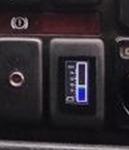
\includegraphics[width=.85\textwidth,height=.60\textheight,keepaspectratio]{figures/ivevo/image16.png}
\caption{IV-Evo Voltmeter}
\end{figure}
\begin{figure}[htbp]
\centering
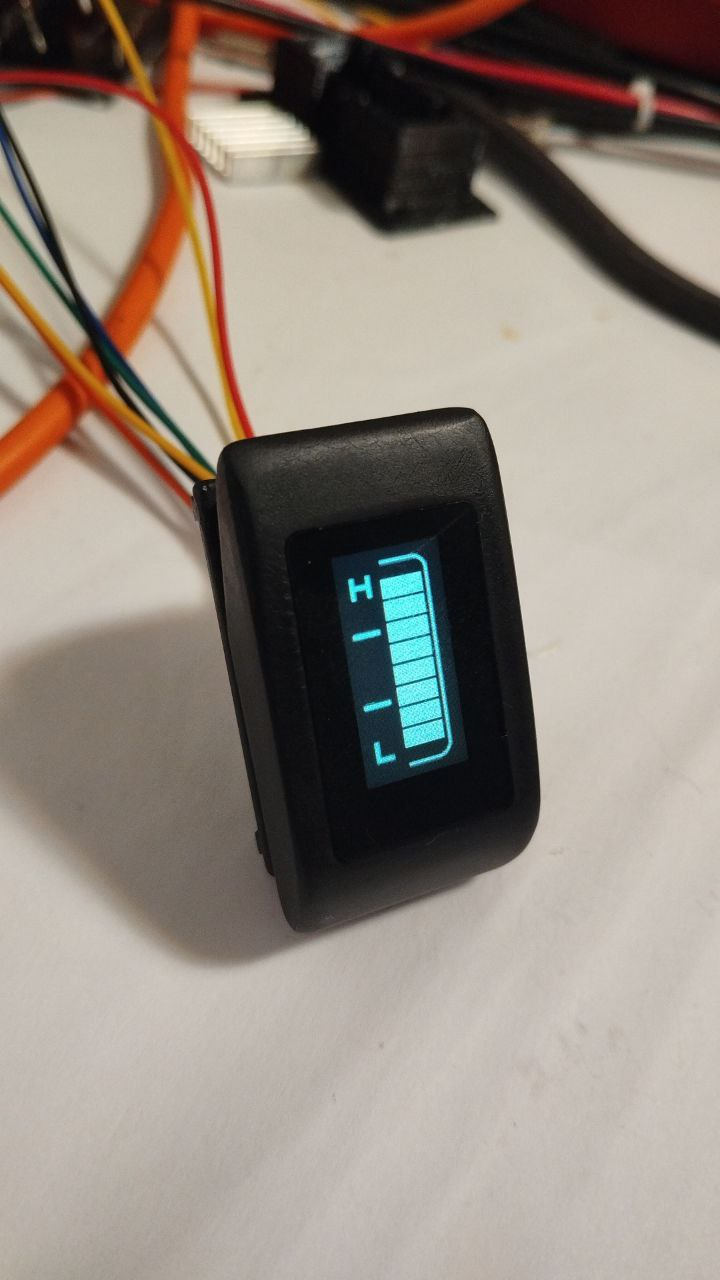
\includegraphics[width=.85\textwidth,height=.60\textheight,keepaspectratio]{figures/ivevo/image15.png}
\caption{IV-Evo Voltmeter}
\end{figure}
\begin{figure}[htbp]
\centering
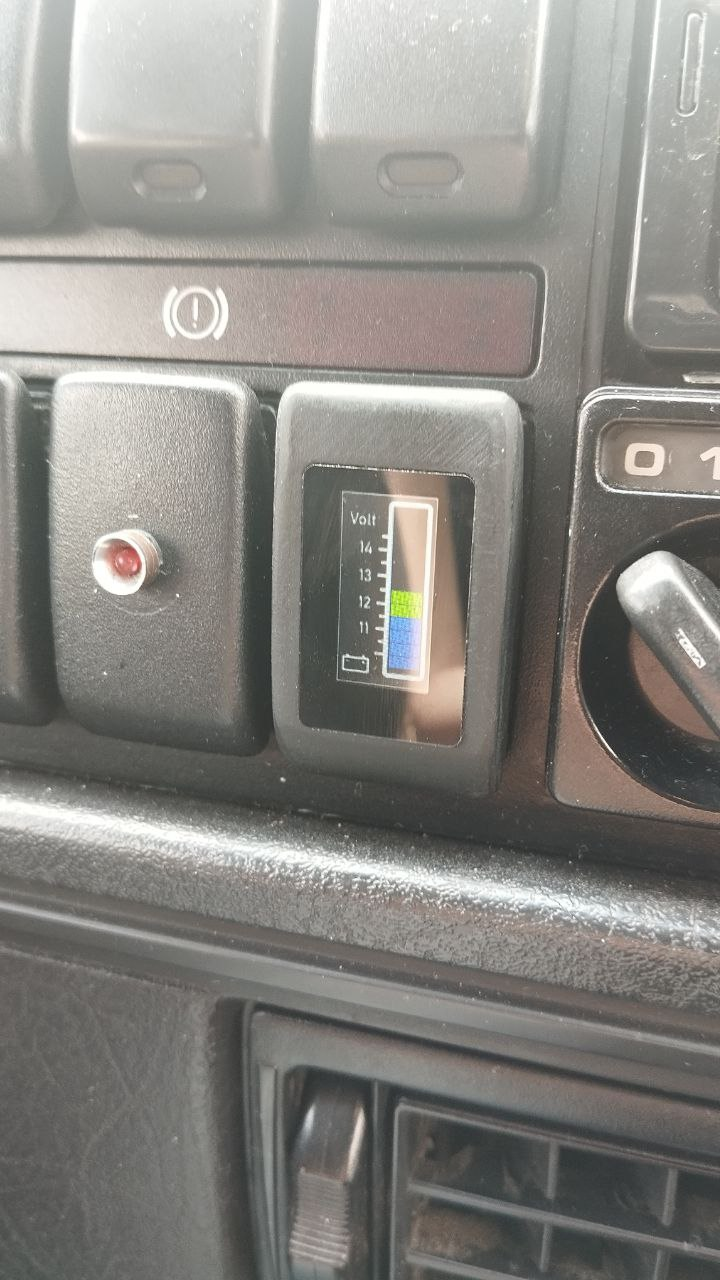
\includegraphics[width=.85\textwidth,height=.60\textheight,keepaspectratio]{figures/ivevo/image2.png}
\caption{IV-Evo Voltmeter}
\end{figure}
IV-Evo voltmeter application type allows you to show the car battery voltage while you are driving.

Applications for the voltmeter:

evo\_v\_l

Displays voltage readings. Includes text voltage and a dedicated background image for voltage monitoring (“battery” icon)

iv\_evo\_v\_t

Displays voltage readings in segments-way like an IV-Nano

\section{IV-Evo  Barometer}
IV-Evo  barometer allows to show car oil pressure while you are driving. Sensor installation is mandatory

IV-Evo  Barometer is intended to be working with VAG pressure sensor p.No 03C906051A

Even though IV-Evo has its own +5V source, it’s still recommended to use external DC/DC for the power.

\section{IV-Evo Thermo}
There are actually two sensor options for IV-Evo Thermo. You can use either NTC or DS18B20 digital sensor.

If thermometer app uses DS18B20 digital sensor to check the temperature in certain location, cables like on the photo are supported, or any other DS18B20 assemblies.

\begin{figure}[htbp]
\centering
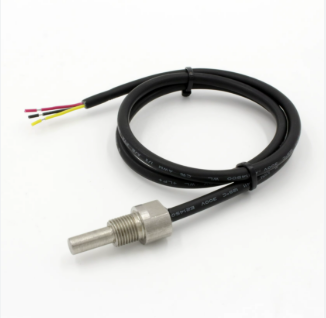
\includegraphics[width=.85\textwidth,height=.60\textheight,keepaspectratio]{figures/ivevo/image14.png}
\caption{IV-Evo Thermo}
\end{figure}
Figure. DS18B20 with bulb and cable

In case of NTC sensor, the following one is recommended:

Ossca 01176

\begin{figure}[htbp]
\centering
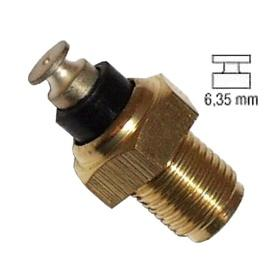
\includegraphics[width=.85\textwidth,height=.60\textheight,keepaspectratio]{figures/ivevo/image19.jpg}
\caption{IV-Evo Thermo}
\end{figure}
On the Ossca sensor, join sensor pins 1 and 2; the NTC resistance is connected to sensor pin 3. These are sensor pin numbers, not the indicator power pins.

\section{IV-Evo Gear indicator}
IV-Evo Gear is a gearbox selected gear indicator, supporting R, 1,2,3,4,5 gears

The idea beyond the indicator is to calculate the gear based on current speed and RPM. Reverse gear is shown if the sensor has positive input on one of inputs.

Device is operated with Bluetooth, and you’ll need Digifiz Next unit in your car for correct operation. Also, speedometer and RPM, as well as gear table should be calibrated to match.

To use IV-Evo Gear, you need to just power it up using pins 1 and 7 (KL30 pin - connect to KL15, ignition power, pin 7 - connect to ground) After that, device will power up and show “-” - meaning that gear is not selected.

Device takes its data from Bluetooth channel from Digifiz Next, so right after the starts its search for Digifiz Next unit.

You’ll need to update your Digifiz Next to a firmware not less than 1.0.14 version, which  introduces BLE streaming of several parameters.

\begin{figure}[htbp]
\centering
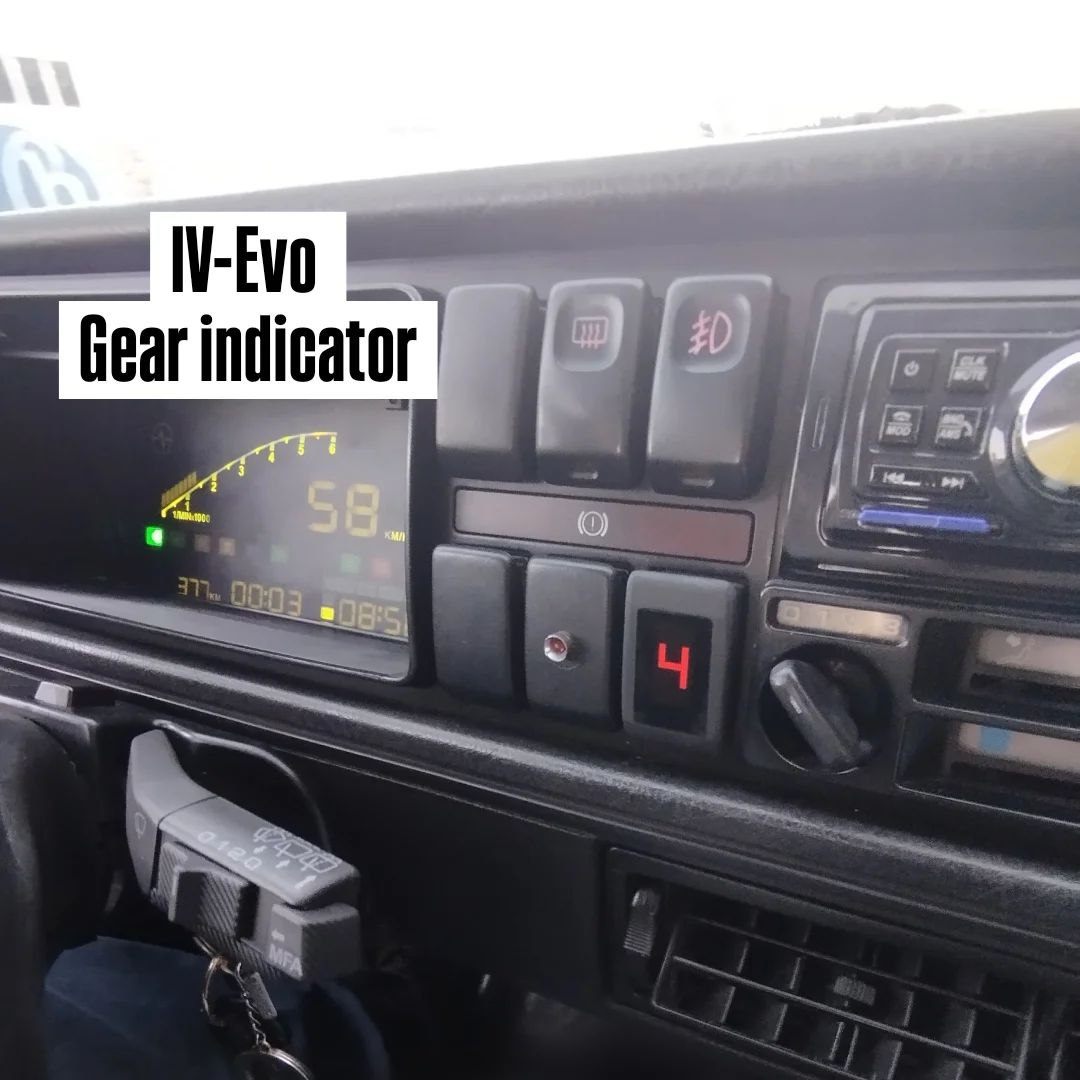
\includegraphics[width=.85\textwidth,height=.60\textheight,keepaspectratio]{figures/ivevo/image18.png}
\caption{IV-Evo Gear indicator}
\end{figure}
\begin{figure}[htbp]
\centering
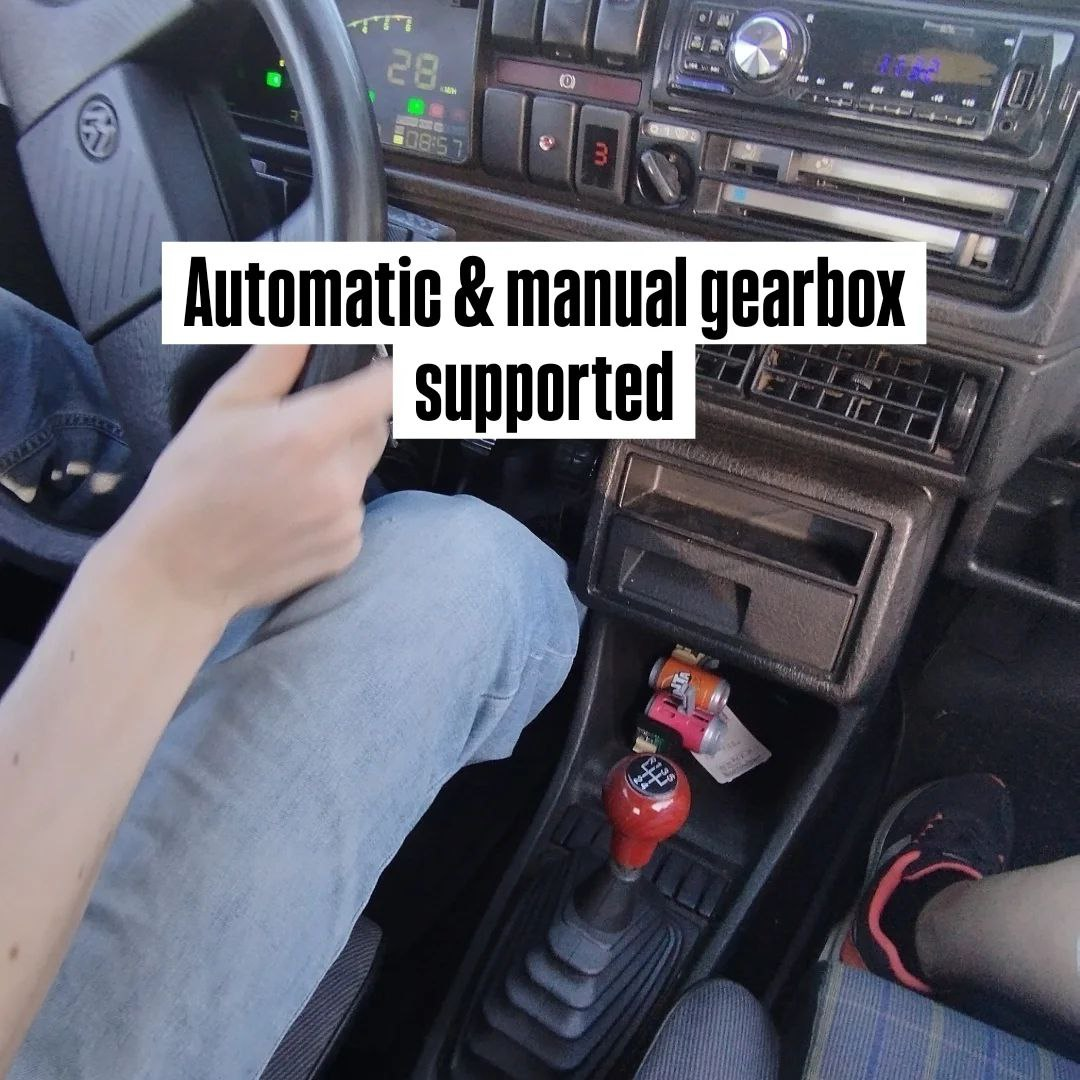
\includegraphics[width=.85\textwidth,height=.60\textheight,keepaspectratio]{figures/ivevo/image10.png}
\caption{IV-Evo Gear indicator}
\end{figure}
Installation guide:

\begin{enumerate}
\item Install Digifiz Next v1.0.14 to your dashboard
\item Connect power +12V KL15 ignition and car masse to pin 1 and pin 7 accordingly
\item Power on in a boot mode(press boot button shortly after turn on) - QR Code will appear. Scan it from you phone and connect to the dashboard.
\item Select application and sensor - “iv\_gear” and “volts1”, save selection
\item Restart by ignition off and on
\item Preliminary installation is complete!
\end{enumerate}
After that, you’ll need to perform a tuning of parameters on Digifiz Next cluster Wi-Fi control panel.

\begin{enumerate}
\item First of all, calibrate your speed using GPS speed from your phone, use 80--100 km/h as a reference only where lawful and safe, with a passenger recording readings.
\end{enumerate}
The parameter for speed calibration is on the Settings page.

\begin{enumerate}
\item After that, calibrate RPM setting by using the same settings page. The source mentions calibration values 1500, 3000 and 400 but does not define their units or map them unambiguously to engines. Use the Digifiz Next instructions for the actual engine rather than selecting an arbitrary value. The speed, RPM and gear table must all match the vehicle.
\end{enumerate}
\section{IV-Evo Lambda}
\begin{figure}[htbp]
\centering
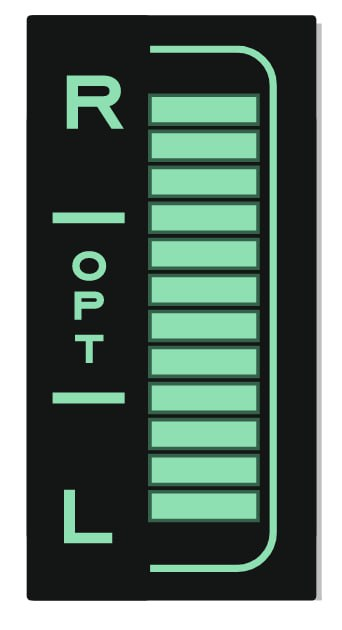
\includegraphics[width=.85\textwidth,height=.60\textheight,keepaspectratio]{figures/ivevo/image7.png}
\caption{IV-Evo Lambda}
\end{figure}
For IV-Evo Lambda the connection is somewhat more complicated.

It is important that connection to stock Golf 2 lambda sensor is not possible

Lambda sensor measurement should be done with 2 lambda sensors installed in the car.

There are two types of Lambda sensors:

Narrowband Oxygen Sensor:

\begin{itemize}
\item Operation: Measures only whether the air-fuel mixture is rich or lean.
\item Output: Produces a voltage between 0.1V (lean) and 0.9V (rich), without detailed information on the exact air-fuel ratio.
\item Use: Common in older vehicles for basic emissions control.
\end{itemize}
Wideband Oxygen Sensor:

\begin{itemize}
\item Operation: Provides precise measurements of the actual air-fuel ratio over a wide range, not just rich or lean.
\item Output: Delivers a linear signal, giving the engine control unit detailed feedback to optimize fuel injection.
\item Use: Found in modern vehicles for more accurate fuel management and emissions control.
\end{itemize}
The problem is that narrowband sensors are not applicable for most of custom engines and carburetors, only wideband ones. And they are more advanced, require more control operations. The indicator itself cannot control wideband sensor, and works directly only with narrowband sensors(needs to be calibrated though)

However, installation of wideband sensor is possible and recommended. For wideband sensor we do recommend Bosch LSU 4.9 sensor, which should be accompanied with supported wideband controller:

\begin{itemize}
\item SLC Free
\item DIY-EFI TinyWB Wideband controller
\item Sigma Lambda Controller Free 2
\item rusEFI wideband lambda
\item Others
\end{itemize}
After buying such wideband controller please connect it according to its diagram to LSU 4.9 and use analog output (typically, 0-5V, 0.5-4.5 or even 0-1V output) for connection to the IV-Indicator Lambda. Below, on connection diagrams, you can find an example connection.

\section{IV-Evo Check Engine}
\begin{figure}[htbp]
\centering
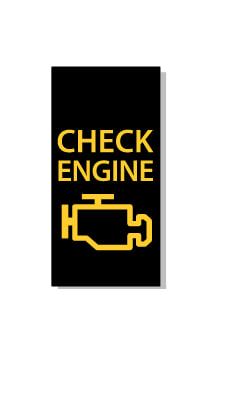
\includegraphics[width=.85\textwidth,height=.60\textheight,keepaspectratio]{figures/ivevo/image4.png}
\caption{IV-Evo Check Engine}
\end{figure}
IV Evo Check Engine is a check engine indicator for your car. It displays “Check engine” or empty screen depending on pin 2 - V2, state. If it’s 12V - Check Engine is displayed, if 0V - nothing is displayed.

\section{IV-Evo Boost}
IV-Evo Boost displays boost pressure while driving. Sensor installation is mandatory

The following sensor is recommended for the installation:

\begin{figure}[htbp]
\centering
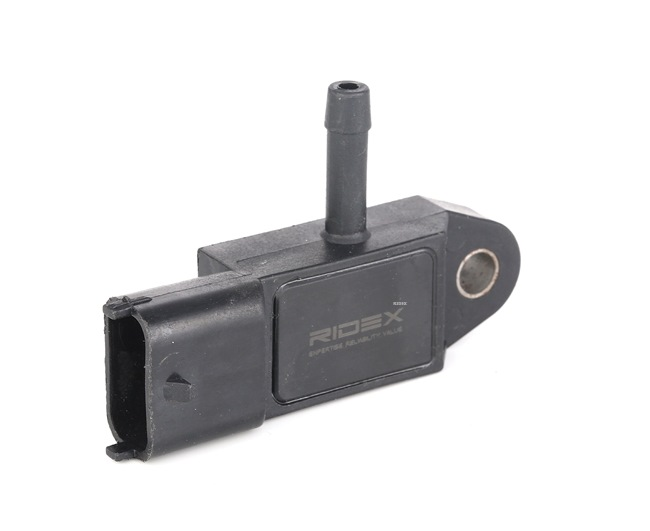
\includegraphics[width=.85\textwidth,height=.60\textheight,keepaspectratio]{figures/ivevo/image9.png}
\caption{IV-Evo Boost}
\end{figure}
Boost sensor characteristics:

\begin{itemize}
\item Number of pins:3
\item Power voltage: +5 V
\item Number of mounting bores:1
\item Pressure from [kPA]:20
\item Pressure to [kPA]:250
\item Nominal sensor output voltage: +1.8V
\end{itemize}
\section{IV-Evo Clock}
\begin{figure}[htbp]
\centering
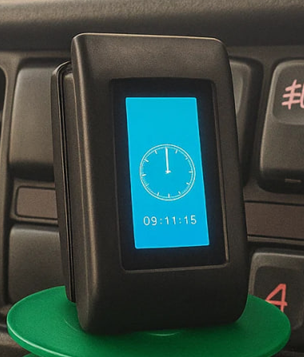
\includegraphics[width=.85\textwidth,height=.60\textheight,keepaspectratio]{figures/ivevo/image12.png}
\caption{IV-Evo Clock}
\end{figure}
IV-Evo clock is an example app which works like a system clock of the indicator. Works like a bootstrap app for the indicator. However, the time is not saved on boot, so it only acts as trip time indicator in that case.


\section{Calibration limits in the reference}
The boost sensor description does not provide a full voltage-to-pressure transfer function or identify the pressure at its nominal +1.8 V output. Confirm the exact sensor and calibration curve before setting the scale. The reference gives no general enclosure ingress rating, operating temperature range or supply voltage tolerance; do not assume Nano specifications apply.
